%\documentclass[twoside, 12pt]{book}
\documentclass[twoside, 11pt]{article}
\usepackage[english]{babel}
\usepackage{epsfig}
\usepackage{psfig}
\usepackage{amssymb,amsmath,amsfonts,soul,amsthm,enumerate}
\usepackage{graphicx}
\usepackage[utf8]{inputenc}
\usepackage[T1]{fontenc}
\usepackage{mathrsfs}
\usepackage{hyperref}
\usepackage{orcidlink}
\textwidth=155mm
\textheight=233mm
\voffset=-15mm
\oddsidemargin=12.1mm
\evensidemargin=-9.1mm
\graphicspath{{figures/}}
\newtheorem{theorem}{Theorem}[section]
\newtheorem{definition}{Definition}
\newtheorem{statement}{Statement}[section]
\newtheorem{lemma}{Lemma}[section]
\newtheorem{corollary}{Corollary}[section]
\newtheorem{proposition}{Proposition}[section]
\newtheorem{remark}{Remark}
\newtheorem{property}{Property}

\pagestyle{myheadings}
\makeatletter
\def\@evenfoot{}
\def\@oddfoot{}
\makeatother

\markboth{\hfill{\footnotesize\rm Koshikov and Tutkyshbayeva}\hfill}
{\hfill{\footnotesize\sl Policy-guided virtual mentor model}\hfill}

\begin{document}
\makeatletter
\def\@evenhead{\vbox{\hbox to \textwidth{\thepage\leftmark}\strut\newline\hrule}}
\def\@oddhead{\raisebox{0pt}[\headheight][0pt]{%
\vbox{\hbox to \textwidth{\rightmark\thepage\strut}\hrule}}}
\makeatother

\newpage
\normalsize
\def\bibname{\vspace*{-30mm}{\centerline{\normalsize References}}}
\thispagestyle{empty}
\begin{flushleft}
{\small {\bf EURASIAN JOURNAL OF MATHEMATICAL \\ AND COMPUTER APPLICATIONS}\\
ISSN 2306--6172\\
Volume 14, Issue (2026) \_ -- \_}
\end{flushleft}
\vskip 5 mm

\centerline{\bf A POLICY-GUIDED VIRTUAL MENTOR MODEL}
\centerline{\bf FOR REAL-TIME FEEDBACK TO FIRST-YEAR PROGRAMMING STUDENTS}

\vskip 0.2cm
\centerline{\bf Koshikov A. \orcidlink{0009-0003-3234-6487}, Tutkyshbayeva S. \orcidlink{0000-0002-1419-2571}}

\vskip 0.2cm
\noindent{\bf Abstract}
{\small
Real-time programming mentors often fail in one of two ways: they either return generic automated feedback or give too much help through an unconstrained language model. This paper presents a policy-guided virtual mentor model for first-year programming students. The model separates code analysis, lightweight student-state tracking, feedback-action selection, and message realization. The main machine learning task is formulated as four-class pedagogical action selection: code highlight, conceptual hint, guiding question, or no feedback. The implementation, SocratesAI, was evaluated with a controlled 12-problem benchmark, a 381003-row weak-label policy corpus, and a 60564-row auxiliary Codeforces submission corpus. In the fixed ML and Gemini runtime benchmark, the system processed 360 events with 0 runtime errors, 95.83\% agreement, 95.80\% macro F1, and 1079.21 ms mean latency. Ablation results show that analyzer-derived features are essential for policy prediction.
\vskip 0.2cm
\noindent {\bf Key words:} virtual mentor, programming education, policy learning, real-time feedback, student modeling, machine learning
\vskip 0.2cm
\noindent {\bf AMS Mathematics Subject Classification:} 68T05, 68T07, 68T10, 62H30}

\vskip 0.2cm
\noindent {\bf DOI:} to be assigned
\vskip 0.3cm
\setcounter{figure}{0}

\section{\large Introduction}

Introductory programming is difficult for many first-year students not because every task is algorithmically complex, but because small mistakes appear at the wrong moment. A missing statement ending, a wrong loop boundary, an unfinished branch, or a condition that never becomes false can stop the whole problem-solving process. In a laboratory class, a teaching assistant can usually ask one short question and bring the student back to work. At scale, this does not happen consistently. Automated assessment systems and unit tests are useful, but they often say only that the program is wrong. A general language-model assistant can be more fluent, but it may reveal too much and change the task from programming practice into answer retrieval.

This paper studies a narrower and more researchable version of the virtual mentor problem. The goal is not to build a general chatbot for programming. The goal is to decide what type of pedagogical intervention is appropriate for the current code state and the current short-term student state. In this formulation, feedback generation is not the central machine learning task. The central task is feedback-action selection under real-time constraints.

The proposed system, SocratesAI, implements this idea as a four-stage pipeline. A code analyzer first extracts structured signals from the current program. A lightweight session state then records repeated errors and recent feedback history. A policy model selects one of four bounded actions: \texttt{CODE\_HIGHLIGHT}, \texttt{CONCEPTUAL\_HINT}, \texttt{GUIDING\_QUESTION}, or \texttt{NO\_FEEDBACK}. Only after this action is selected is a template or language model allowed to phrase the student-facing message. This separation is important because it makes the mentoring decision auditable. The language model can realize a selected intervention, but it does not control the tutoring strategy.

The research questions are:
\begin{enumerate}
\item Can a policy-guided mentor operate within an interactive latency range during programming practice?
\item How accurately can the implemented policy select rubric-aligned feedback actions on controlled CS1-style code states?
\item Do analyzer-derived features contribute measurable signal to feedback-action prediction?
\item Which external programming-submission dataset is most suitable as an auxiliary corpus for future policy validation?
\end{enumerate}

The contribution of the paper is fourfold. First, a formal policy-guided model of real-time programming mentoring is proposed. Second, an implemented Spring Boot, PostgreSQL, Vue, and FastAPI prototype is described as a running decision system rather than only as a web application. Third, the evaluation combines runtime benchmarks, policy model comparison, and feature ablation. Fourth, three HuggingFace Codeforces datasets are inspected, and the most suitable subset is converted into an auxiliary 60564-row policy dataset for external consistency checking.

\section{\large Related Work and Research Gap}

Automated feedback for programming education has been studied through compilers, unit tests, static analysis, program repair, and intelligent tutoring systems. Recent systematic reviews show that such systems can provide scalable support, but many tools remain focused on correctness and grading instead of the level of help that should be given to a learner at a particular moment \cite{messer2024,kumar2025}. Immediate adaptive feedback systems address part of this limitation by connecting interventions to subgoals and learner progress \cite{marwan2022}. Fuzzy and adaptive tutoring approaches also demonstrate the value of explicit learner modeling in programming education \cite{chrysafiadi2023}. However, these systems are often evaluated at coarser interaction points than active code editing.

The second relevant line of work is AI-assisted programming feedback. Studies of LLM-based assistants such as CodeAid, Iris, CS50 AI, and related tools show that fluent explanations can be useful when they are constrained by educational design \cite{denny2024,kazemitabaar2024,bassner2024,liu2025}. At the same time, classroom and help-seeking studies report risks: students may ask for the next answer too quickly, accept confident but incomplete explanations, or use the assistant in ways that reduce productive struggle \cite{sheese2024,ahmed2025}. For this reason, the important design question is not only whether a model can generate feedback. It is whether the system can regulate the amount, timing, and type of help before the text is generated.

Recent work on tutor-style feedback generation uses large models for hint production and validation \cite{phung2024}, and studies of LLM feedback generation in programming courses show that generated feedback must be evaluated carefully against course context \cite{estevez2025,pankiewicz2023}. SocratesAI is positioned between these directions. It does not attempt to replace a full intelligent tutor, and it does not rely on open-ended chat. Its research gap is policy-level control: a compact decision model selects the pedagogical action, while feedback wording remains a separate realization step.

\section{\large Policy-Guided Mentor Model}

\subsection{Event Representation}

Let $c_t$ denote the student's code state at interaction time $t$. The analyzer maps this code state to a structured event descriptor
\begin{equation}
e_t = A(c_t),
\end{equation}
where $e_t$ contains compile status, error type, severity, estimated tests passed and failed, code length, and suspicious-region information. The current implementation focuses on novice-relevant states such as syntax errors, unfinished implementation, off-by-one patterns, wrong loop boundaries, missing guards, possible infinite loops, and unknown logic blocks.

The short-term student state is represented as
\begin{equation}
s_t = (r_t, n_t, b_t, u_t, f_t),
\end{equation}
where $r_t$ is the current repeated-error count, $n_t$ is the number of recent errors in the session, $b_t$ is the last feedback action, $u_t$ is the previous feedback success flag, and $f_t$ is the total feedback count in the current session. This is not a full knowledge tracing model. It is intentionally small because the target interaction is a short programming session, not a semester-long cognitive model.

The feature vector used by the policy is
\begin{equation}
x_t = \phi(e_t, s_t, q_t),
\end{equation}
where $q_t$ contains attempt-level metadata such as attempt number and task context. In the implementation, $x_t$ has categorical, Boolean, and numeric features. Categorical values include error type, severity, and previous action. Boolean values include compile success and suspicious-region presence. Numeric values include passed tests, failed tests, repeated-error count, total errors seen, attempt number, code lines, and total feedback count in the session.

\subsection{Action Space}

The mentor policy selects an action from the finite set
\begin{equation}
\mathcal{A} =
\{\mathrm{HL}, \mathrm{CH}, \mathrm{GQ}, \mathrm{NF}\},
\end{equation}
where $\mathrm{HL}$ is code highlight, $\mathrm{CH}$ is conceptual hint, $\mathrm{GQ}$ is guiding question, and $\mathrm{NF}$ is no feedback. The actions are ordered informally by intervention style, not by correctness. A code highlight points to a location with minimal explanation. A conceptual hint gives a short idea. A guiding question asks the student to inspect or explain part of the code. No feedback is selected when the system should stay silent.

The policy is therefore
\begin{equation}
\pi_{\theta}: x_t \rightarrow a_t,\quad a_t \in \mathcal{A}.
\end{equation}
For supervised learning, the parameter $\theta$ is estimated by minimizing empirical classification loss
\begin{equation}
\hat{\theta} =
\arg \min_{\theta}
\frac{1}{N}\sum_{i=1}^{N} L(y_i,\pi_{\theta}(x_i)),
\end{equation}
where $y_i$ is a target feedback action. In the current experiments, $y_i$ comes from either an explicit problem-suite rubric or weak labels derived from policy behavior or judge verdicts. This distinction is important because weak labels are useful for scale and ablation, but they are not equivalent to instructor-labelled classroom feedback.

\subsection{Feedback Realization}

The final message is generated by a realization function
\begin{equation}
m_t = G(a_t,e_t,c_t),
\end{equation}
with the constraint that $m_t$ should not disclose a full corrected solution. The current implementation supports deterministic templates and an optional LLM realization path. In the LLM path, the selected action is fixed before the prompt is constructed. Thus the LLM phrases a bounded intervention rather than deciding the tutoring strategy.

The total latency is decomposed as
\begin{equation}
T_t = T^{A}_t + T^{S}_t + T^{\pi}_t + T^{G}_t + T^{O}_t,
\end{equation}
where $T^{A}_t$ is analyzer time, $T^{S}_t$ is session-state time, $T^{\pi}_t$ is policy time, $T^{G}_t$ is feedback realization time, and $T^{O}_t$ is platform overhead. This decomposition is used because a real-time mentor must be evaluated as an interactive system, not only as an offline classifier.

\begin{figure}[t]
\centering
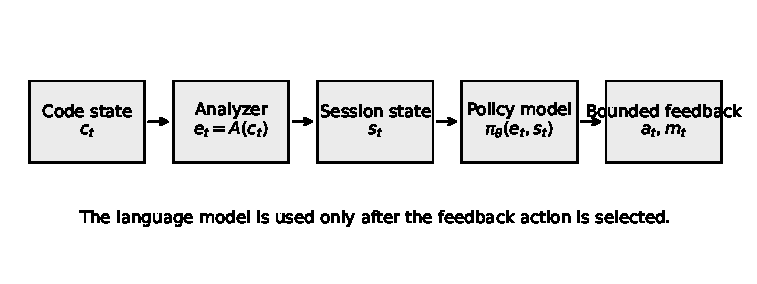
\includegraphics[width=120mm]{Figure1_policy_pipeline.pdf}
\caption{Policy-guided mentoring pipeline. The LLM, when enabled, is used after action selection.}
\label{fig:pipeline}
\end{figure}

\section{\large Implementation}

SocratesAI is implemented as a full-stack prototype. The backend is written in Java 21 with Spring Boot. The frontend is a Vue 3 application with a code editor and mentor feedback panel. PostgreSQL stores users, tasks, sessions, and interaction logs. A FastAPI service serves the optional ML policy model. The core backend modules are separated into analyzer, mentor, policy, feedback, interaction logging, session, task, user, security, and WebSocket packages.

The analyzer combines a Java syntax check with lightweight pattern detection. Syntax errors are detected through the Java compiler API where available, with a fallback heuristic path. Pattern detection identifies beginner-level signals such as unfinished implementation, suspicious loop boundaries, possible null or empty-guard issues, and wrong conditions. The analyzer is deliberately not presented as a complete program-understanding engine. Its role is to produce structured signals that are useful for policy selection.

The session context is built from recent interaction logs. For each event, the backend stores the selected feedback action, feedback source, policy version, timing components, compile status, tests passed, tests failed, suspicious-region flag, code hash, feedback-helpfulness fields, and outcome fields. Raw code is not stored in the interaction log table; a code hash is stored for traceability with lower privacy risk.

The policy layer supports three modes. In rule mode, a deterministic policy maps analyzer and session features to one of the four actions. In ML mode, the backend sends a snake-case JSON feature vector to the FastAPI policy service and applies a guardrail layer after prediction. In no-policy mode, the system always returns a conceptual hint, which is used as a weak baseline. If the ML service fails and fallback is enabled, the backend returns to the rule policy.

The deployed classifier is a Random Forest with 200 trees, maximum depth 8, minimum leaf size 2, and balanced subsampling. The preprocessing pipeline imputes missing values and one-hot encodes categorical features. Additional experiments compare Logistic Regression, Random Forest, XGBoost, LightGBM, and a small neural classifier. Standard implementations from scikit-learn, XGBoost, and LightGBM are used \cite{breiman2001,pedregosa2011,chen2016,ke2017}.

\section{\large Datasets and Experimental Design}

\subsection{Dataset Selection}

Three local HuggingFace datasets were inspected. The first Codeforces Python dataset contains Python submissions, problem statements, prompt/response fields, verdicts, and passed-test counts. It is useful for code generation and Python-focused reasoning, but it is less aligned with the current Java-oriented CS1 mentor. The second user-history dataset contains anonymized user trajectories, ratings, problem ratings, verdicts, and timestamps. It is useful for long-term recommendation and progression modeling, but it does not contain source code. The third open-r1 Codeforces submissions dataset contains real human submissions with source code, verdict, passed-test count, problem id, language, time, and memory. Its \texttt{selected\_accepted} and \texttt{selected\_incorrect} subsets were therefore chosen as the most suitable auxiliary corpus for this paper \cite{penedo2025}.

The selected Codeforces corpus is not treated as classroom data. It is competitive-programming data and includes many languages. Its value here is narrower: it gives an external human-submission corpus from which verdict-derived policy labels can be constructed. Accepted submissions map naturally to \texttt{NO\_FEEDBACK}. Compilation and runtime failures map to localized interventions. Wrong-answer and time-limit cases map to conceptual or guiding support depending on passed-test count and verdict. This produces weak labels, not instructor labels.

\begin{table}[t]
\centering
\caption{Evaluation and Training Artifacts}
\label{tab:artifacts}
\small
\begin{tabular}{p{38mm}p{22mm}p{77mm}}
\hline
\textbf{Artifact} & \textbf{Size} & \textbf{Role in the study} \\
\hline
Real HTTP replay & 570 events & Backend and PostgreSQL responsiveness in deterministic feedback mode. \\
Stress smoke test & 400 requests & Stability under eight-way concurrent local load. \\
Problem-suite rubric dataset & 1080 rows & Main supervised action-selection dataset with target feedback actions. \\
Fixed ML and Gemini benchmark & 360 events & End-to-end benchmark with ML policy, PostgreSQL state, and LLM realization. \\
Expanded weak-label corpus & 381003 rows & Scale check, model comparison, and feature ablation. \\
Codeforces auxiliary corpus & 60564 rows & External human-submission consistency check based on verdict-derived weak labels. \\
\hline
\end{tabular}
\end{table}

\subsection{Problem-Suite Benchmark}

The controlled problem suite contains 12 programming tasks: palindrome checking, two-sum, valid parentheses, binary search, merge sorted array, trapping rain water, LRU cache, longest substring without repeating characters, reverse linked list, matrix diagonal sum, Roman-to-integer conversion, and climbing stairs. Each task is replayed as a six-state sequence: syntax issue, unfinished implementation, first conceptual mistake, repeated conceptual mistake, partial compiling logic, and local completion. A target feedback action is assigned by a review rubric.

The fixed runtime benchmark used Docker Compose, PostgreSQL, the Spring Boot backend, the FastAPI ML policy service, fresh student identifiers, and Gemini 2.5 Flash-Lite feedback realization. Earlier ML runs that used contaminated student histories or an unsafe backend-to-ML JSON contract are not used as primary evidence.

\subsection{Metrics}

For a class $k$, precision, recall, and F1 are defined as
\begin{equation}
P_k=\frac{TP_k}{TP_k+FP_k},\quad
R_k=\frac{TP_k}{TP_k+FN_k},\quad
F1_k=\frac{2P_kR_k}{P_k+R_k}.
\end{equation}
The macro F1 score is
\begin{equation}
F1_{\mathrm{macro}}=\frac{1}{|\mathcal{A}|}\sum_{k \in \mathcal{A}} F1_k.
\end{equation}
In addition to accuracy and macro F1, the evaluation reports runtime errors, mean latency, P95 latency, feedback source, action distribution, per-problem agreement, and ablation results.

\section{\large Results}

\subsection{Backend Responsiveness}

The real-HTTP PostgreSQL replay processed 570 requests with 0 errors. Mean request latency was 44.11 ms, median latency was 46 ms, P95 latency was 58 ms, and P99 latency was 68 ms. Analyzer time averaged 6.81 ms. Under an additional 400-request stress smoke test with concurrency 8, all requests completed successfully. Mean latency was 37.59 ms, P95 latency was 56 ms, and throughput was 211.19 requests per second. These numbers show that the deterministic core mentoring loop is fast enough for interactive use.

\subsection{End-to-End ML and LLM Benchmark}

The primary runtime result is the fixed ML and Gemini benchmark. The system processed 360 events across 12 problems and five cohorts with 0 runtime errors. Agreement with the target feedback action was 95.83\%, and macro F1 was 95.80\%. Mean wall latency was 1079.21 ms and P95 latency was 2072 ms. Gemini produced 317 responses, while 43 responses used deterministic template fallback.

\begin{table}[t]
\centering
\caption{Fixed ML and Gemini Runtime Benchmark}
\label{tab:runtime}
\small
\begin{tabular}{lc}
\hline
\textbf{Metric} & \textbf{Value} \\
\hline
Events & 360 \\
Successful requests & 360 \\
Runtime errors & 0 \\
Agreement with target action & 95.83\% \\
Macro F1 & 95.80\% \\
Mean latency & 1079.21 ms \\
P95 latency & 2072 ms \\
Gemini responses & 317 \\
Template fallbacks & 43 \\
\hline
\end{tabular}
\end{table}

\begin{table}[t]
\centering
\caption{Per-Class Action Metrics in the Fixed Runtime Benchmark}
\label{tab:perclass}
\small
\begin{tabular}{lcccc}
\hline
\textbf{Action} & \textbf{Precision} & \textbf{Recall} & \textbf{F1} & \textbf{Support} \\
\hline
\texttt{CODE\_HIGHLIGHT} & 95.24 & 100.00 & 97.56 & 100 \\
\texttt{CONCEPTUAL\_HINT} & 93.10 & 96.43 & 94.74 & 140 \\
\texttt{GUIDING\_QUESTION} & 100.00 & 100.00 & 100.00 & 60 \\
\texttt{NO\_FEEDBACK} & 100.00 & 83.33 & 90.91 & 60 \\
\hline
\end{tabular}
\end{table}

\begin{figure}[t]
\centering
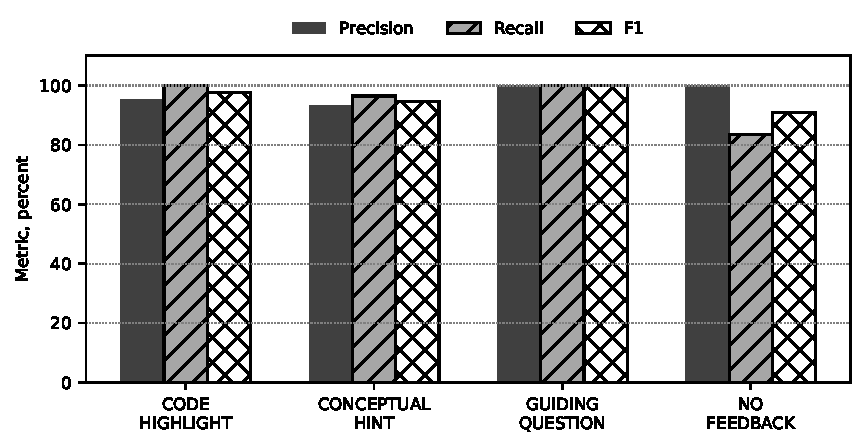
\includegraphics[width=120mm]{Figure2_per_class_metrics.pdf}
\caption{Precision, recall, and F1 by feedback action in the fixed runtime benchmark.}
\label{fig:perclass}
\end{figure}

The weakest class was \texttt{NO\_FEEDBACK}. The system sometimes gave a hint when local completion should have remained silent. This error is pedagogically important: too much help can be as harmful as too little help in a practice setting. The disagreements were concentrated in \texttt{lru-cache} and \texttt{valid-parentheses}, especially local-completion and first conceptual-error states.

\begin{figure}[t]
\centering
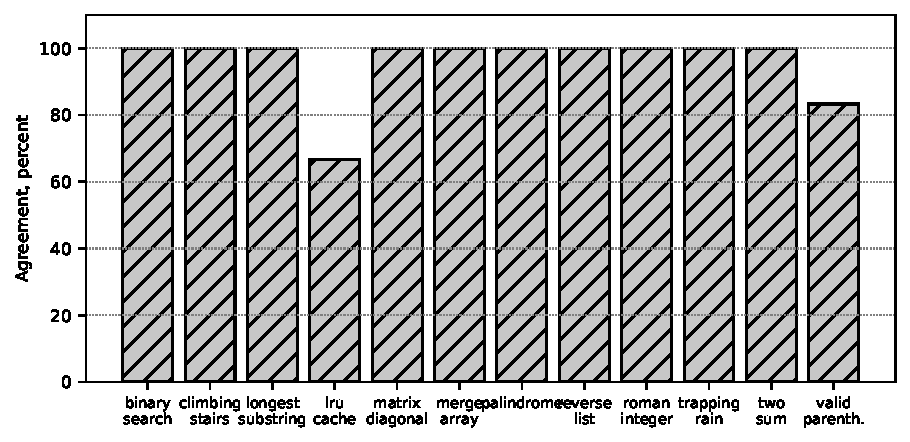
\includegraphics[width=120mm]{Figure3_problem_agreement.pdf}
\caption{Agreement with target feedback action by programming problem.}
\label{fig:problems}
\end{figure}

\subsection{Model Comparison and Ablation}

The 1080-row problem-suite dataset was evaluated with a problem-level group holdout. The Random Forest classifier trained on 810 rows and tested on 270 rows from held-out problems. It reached 1.0000 accuracy and 1.0000 macro F1. This result means that the rubric mapping is learnable from the exported runtime features; it does not prove that the system improves learning outcomes.

The expanded weak-label corpus contains 381003 rows from 117232 coding sessions. On this corpus, several model families reproduced the weak policy labels with 1.0000 macro F1. The more informative result is the ablation. Removing analyzer-derived features reduced macro F1 to 0.8813. On the auxiliary Codeforces corpus, the same ablation reduced Random Forest macro F1 to 0.4782, even though all features produced 1.0000 macro F1. This supports the architectural claim that structured analyzer signals are not decorative. They carry the main information needed for policy-action selection.

\begin{table}[t]
\centering
\caption{Policy Dataset Results and Interpretation}
\label{tab:modelresults}
\small
\begin{tabular}{p{38mm}p{20mm}p{25mm}p{52mm}}
\hline
\textbf{Dataset} & \textbf{Rows} & \textbf{Macro F1} & \textbf{Interpretation} \\
\hline
Problem-suite rubric & 1080 & 1.0000 & Rubric action labels are learnable under problem-level holdout. \\
Expanded weak-label corpus & 381003 & 1.0000 & Large-scale policy imitation and pipeline stability check. \\
Codeforces auxiliary corpus & 60564 & 1.0000 & Verdict-derived weak labels are consistently recoverable from policy features. \\
\hline
\end{tabular}
\end{table}

\begin{figure}[t]
\centering
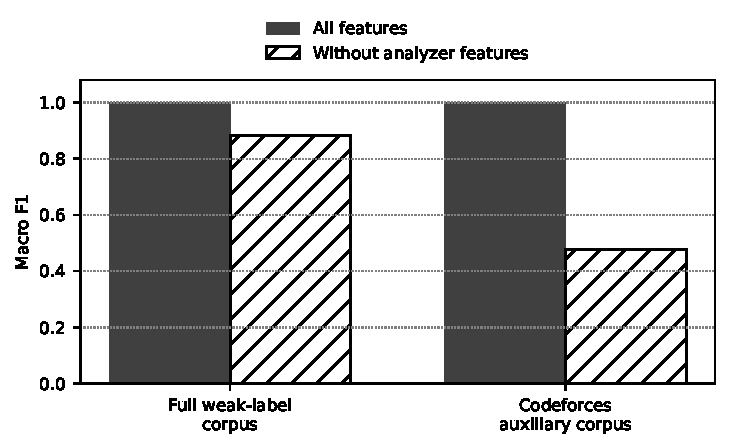
\includegraphics[width=105mm]{Figure4_ablation_macro_f1.pdf}
\caption{Macro F1 with all features and after removing analyzer-derived features.}
\label{fig:ablation}
\end{figure}

\subsection{Baseline Context}

A no-policy baseline that always returns \texttt{CONCEPTUAL\_HINT} reached only 38.89\% agreement and 0.1400 macro F1 in the deterministic 12-problem comparison. This result is simple but useful. It shows why a virtual mentor should not be evaluated only by whether it can generate a fluent message. A generic hint-only system cannot highlight code, ask a question, or stay silent when silence is the best action.

\section{\large Discussion}

The main finding is that SocratesAI is better understood as a policy-controlled decision system than as an AI chat interface. This framing makes the master's thesis deeper because the research object becomes explicit: the action-selection policy, its feature representation, its latency budget, and its error profile. The model does not claim to understand all programs. Instead, it maps novice-relevant analyzer and session signals to bounded pedagogical actions.

The result also explains why the project should focus on the ML and policy layer in the next paper. Frontend screens and generic LLM wording are not enough for a strong EJMCA article. The stronger contribution is the formal decomposition of mentoring into analyzer state, learner context, action policy, and realization. The ablation study gives a concrete technical argument: when analyzer features are removed, macro F1 drops substantially. This is evidence that the project is not only a wrapper around a language model.

The Codeforces dataset selection adds an additional boundary. The selected open-r1 subsets are suitable for external consistency checks because they contain human code, accepted and incorrect submissions, verdicts, passed-test counts, and problem identifiers. However, they are not a substitute for first-year classroom data. They mostly represent competitive programming, and many submissions are in C++ or Python. For that reason, the paper uses them as an auxiliary weak-label corpus and not as primary educational evidence.

The perfect offline scores must be interpreted carefully. In weak-label corpora, high scores are expected because the target labels are derived from a deterministic or semi-deterministic mapping. The valid claim is that the feature pipeline can reproduce the intended action policy at scale and that removing analyzer features hurts this reproduction. The invalid claim would be that the model has proven pedagogical optimality.

\section{\large Limitations and Future Work}

The first limitation is the absence of a real classroom learning-gain study. The current evaluation measures system behavior, action agreement, and policy prediction. It does not prove that students learn more, retain concepts longer, or debug independently after using the mentor. A classroom study should include pre-test, guided practice, post-test, delayed task, and a control condition.

The second limitation is the weakness of the current analyzer. It captures useful beginner-level signals but does not perform deep semantic program analysis. This is acceptable for the present policy study, but future work should add stronger static analysis, test-trace interpretation, and language-specific error localization.

The third limitation is weak labeling. The expanded policy corpus and the Codeforces auxiliary corpus are useful for scale and ablation, but manually reviewed labels are still needed. The next step should be 200--500 instructor-reviewed events, with 50--100 overlapping events labelled by two raters so that inter-rater agreement can be reported.

The fourth limitation is \texttt{NO\_FEEDBACK}. The system still over-intervenes in some local-completion states. This is a research opportunity rather than only an engineering bug, because deciding when to stay silent is one of the most important parts of a learning-support system.

\section{\large Conclusion}

This paper presented a policy-guided virtual mentor model for real-time personalized programming feedback. The core idea is to separate code analysis, short-term student-state tracking, pedagogical action selection, and feedback realization. This separation makes the mentoring decision explicit and auditable.

The implemented system processed 360 fixed ML and Gemini benchmark events with 0 runtime errors, 95.83\% action agreement, 95.80\% macro F1, and mean latency of 1079.21 ms. Offline policy experiments showed that action labels are learnable from the exported feature vectors, while ablation confirmed that analyzer-derived features carry substantial signal. The selected Codeforces auxiliary corpus adds external weak-label validation, but classroom evidence is still required before making learning-gain claims.

\section*{\large Acknowledgement}

This work was carried out as part of the master's degree research at Astana IT University. The authors thank the School of Software Engineering for supporting the development and evaluation of the SocratesAI prototype.

\begin{thebibliography}{99}
\thispagestyle{myheadings}
\vspace*{0mm} \itemsep=-2pt
\footnotesize

\bibitem{messer2024} Messer M., Brown N.C.C., Kolling M., Shi M., {\it Automated grading and feedback tools for programming education: a systematic review}, ACM Trans. Comput. Educ., 24.1 (2024), Article 10.

\bibitem{kumar2025} Kumar S.S., Lones M.A., Maarek M., Zantout H., {\it Navigating the landscape of automated feedback generation techniques for programming exercises}, ACM Trans. Comput. Educ., 25.4 (2025), Article 54.

\bibitem{marwan2022} Marwan S., Akram B., Barnes T., Price T.W., {\it Adaptive immediate feedback for block-based programming: design and evaluation}, IEEE Trans. Learn. Technol., 15.3 (2022), 406--420.

\bibitem{chrysafiadi2023} Chrysafiadi K., Virvou M., Tsihrintzis G.A., Hatzilygeroudis I., {\it Evaluating the user's experience, adaptivity and learning outcomes of a fuzzy-based intelligent tutoring system for computer programming for academic students in Greece}, Educ. Inf. Technol., 28 (2023), 6453--6483.

\bibitem{denny2024} Denny P., MacNeil S., Savelka J., Porter L., Luxton-Reilly A., {\it Desirable characteristics for AI teaching assistants in programming education}, Proc. ITiCSE 2024, ACM, 2024, 408--414.

\bibitem{kazemitabaar2024} Kazemitabaar M., Ye R., Wang X., Henley A.Z., Denny P., Craig M., Grossman T., {\it CodeAid: evaluating a classroom deployment of an LLM-based programming assistant that balances student and educator needs}, Proc. CHI 2024, ACM, 2024, Article 650.

\bibitem{bassner2024} Bassner P., Frankford E., Krusche S., {\it Iris: an AI-driven virtual tutor for computer science education}, Proc. ITiCSE 2024, ACM, 2024, 394--400.

\bibitem{liu2025} Liu R., Zhao J., Xu B., Perez C., Zhukovets Y., Malan D.J., {\it Improving AI in CS50: leveraging human feedback for better learning}, Proc. SIGCSE TS 2025, ACM, 2025, 715--721.

\bibitem{sheese2024} Sheese B., Liffiton M., Savelka J., Denny P., {\it Patterns of student help-seeking when using a large language model-powered programming assistant}, Proc. ACE 2024, ACM, 2024, 49--57.

\bibitem{ahmed2025} Ahmed U.Z., Sahai S., Leong B., Karkare A., {\it Feasibility study of augmenting teaching assistants with AI for CS1 programming feedback}, Proc. SIGCSE TS 2025, ACM, 2025, 11--17.

\bibitem{phung2024} Phung T., Padurean V.A., Singh A., Brooks C., Cambronero J., Gulwani S., Singla A., Soares G., {\it Automating human tutor-style programming feedback: leveraging GPT-4 tutor model for hint generation and GPT-3.5 student model for hint validation}, Proc. LAK 2024, ACM, 2024, 12--23.

\bibitem{estevez2025} Estevez-Ayres I., Callejo P., Hombrados-Herrera M.A., Alario-Hoyos C., Delgado Kloos C., {\it Evaluation of LLM tools for feedback generation in a course on concurrent programming}, Int. J. Artif. Intell. Educ., 35 (2025), 774--790.

\bibitem{pankiewicz2023} Pankiewicz M., Baker R.S., {\it Large language models (GPT) for automating feedback on programming assignments}, Proc. ICCE 2023, APSCE, 2023.

\bibitem{breiman2001} Breiman L., {\it Random forests}, Mach. Learn., 45.1 (2001), 5--32.

\bibitem{pedregosa2011} Pedregosa F., Varoquaux G., Gramfort A., Michel V., Thirion B., Grisel O., Blondel M., Prettenhofer P., Weiss R., Dubourg V., Vanderplas J., Passos A., Cournapeau D., Brucher M., Perrot M., Duchesnay E., {\it Scikit-learn: machine learning in Python}, J. Mach. Learn. Res., 12 (2011), 2825--2830.

\bibitem{chen2016} Chen T., Guestrin C., {\it XGBoost: a scalable tree boosting system}, Proc. 22nd ACM SIGKDD Int. Conf. Knowl. Discov. Data Min., ACM, 2016, 785--794.

\bibitem{ke2017} Ke G., Meng Q., Finley T., Wang T., Chen W., Ma W., Ye Q., Liu T.Y., {\it LightGBM: a highly efficient gradient boosting decision tree}, Adv. Neural Inf. Process. Syst., 30 (2017), 3146--3154.

\bibitem{penedo2025} Penedo G., Lozhkov A., Kydlicek H., Allal L.B., Beeching E., Lajarin A.P., Gallouedec Q., Habib N., Tunstall L., von Werra L., {\it CodeForces submissions dataset}, Hugging Face repository, 2025. Available at: \url{https://huggingface.co/datasets/open-r1/codeforces-submissions}.

\end{thebibliography}

\footnotesize
\noindent
\parbox[t]{75mm}{
Koshikov Alimzhan,\\
School of Software Engineering, Astana IT University,\\
Astana, Kazakhstan,\\
Email: {\tt 225148@astanait.edu.kz}.}
\hfill
\parbox[t]{75mm}{
Tutkyshbayeva Shyryn,\\
School of Software Engineering, Astana IT University,\\
Astana, Kazakhstan,\\
Email: {\tt sh.tutkyshbayeva@astanait.edu.kz}.}

\vspace{3mm}
Received \_\_.\_\_.2026, $\> \> \> $ Accepted \_\_.\_\_.2026, $\> \> \> $ Available online \_\_.\_\_.2026.

\end{document}
